% Informe en APA 7.ª edición — compilar con pdflatex (o XeLaTeX) en Overleaf.
\documentclass[stu,12pt,letterpaper,donotrepeattitle,floatsintext]{apa7}
\usepackage[spanish,es-tabla,es-noshorthands]{babel}
\usepackage[T1]{fontenc}
\usepackage[utf8]{inputenc}
\usepackage{graphicx,tabularx,booktabs,array,enumitem}
\usepackage{xurl}
\renewcommand{\arraystretch}{1.15}
\newcolumntype{L}{>{\raggedright\arraybackslash}X}

\title{Sistema CRM Integrado a un Portal Web para la Gestión Comercial de Rifat Richani Bienes Raíces}
\shorttitle{Sistema CRM inmobiliario}

\begin{document}

\begin{titlepage}
  \centering
  \raggedright
\includegraphics[width=1in]{figuras/logo-ujap.jpg}\par
  \centering\vspace{0.4cm}
  República Bolivariana de Venezuela\\ Universidad José Antonio Páez\\
  Facultad de Ingeniería\\ Sistema de Base de Datos\\ Sección 306C1\par
  \vspace{2.2cm}
  {\Large\bfseries Sistema CRM Integrado a un Portal Web para la Gestión Comercial de Rifat Richani Bienes Raíces\par}
  \vspace{2.2cm}
  \raggedright Docente: Perez, Juan\par
  \vspace{0.8cm}
  \raggedleft
  Ramirez Daniela, C.I 32659238\\
  Vivas Oscar, C.I 31192066\\
  Ramirez Maria, C.I 32658336\\
  Villarroel Sebastian, C.I 32269496\par
  \vspace{1cm}\centering Octubre 23 del 2026\par
\end{titlepage}

\renewcommand{\contentsname}{Índice}
\setcounter{tocdepth}{2}
\tableofcontents
\newpage

\section{Introducción}

El sector inmobiliario depende de la relación con el cliente: una venta o un alquiler se concreta tras semanas de consultas, visitas, ofertas y trámites, y cada uno de esos contactos genera información que debe conservarse para no perder la oportunidad. La gestión de las relaciones con los clientes, conocida como CRM (\textit{Customer Relationship Management}), propone reunir esa información en un solo sistema para que la empresa conozca a sus clientes, les dé seguimiento y mida sus resultados (Buttle \& Maklan, 2019).

Este informe presenta el desarrollo del Sistema CRM integrado al portal web de Rifat Richani Bienes Raíces, una inmobiliaria de Valencia, estado Carabobo. El sistema une dos áreas que comparten una misma base de datos: un portal público, donde los clientes exploran el catálogo de inmuebles, se registran y solicitan información, y un CRM privado, donde los asesores gestionan esos contactos, sus negocios, los inmuebles, las tareas y las estadísticas comerciales.

El documento se organiza según la estructura del proyecto. Primero se expone la problemática que dio origen al sistema; luego se plantean el objetivo general y los cinco objetivos específicos (diagnosticar, determinar, diseñar, codificar y evaluar); y, por último, se describen las cinco fases del proyecto, cada una asociada a un objetivo: diagnóstico, determinación, diseño, codificación y evaluación. Cierran el informe las conclusiones, las recomendaciones y las referencias.

\section{Problemática}

Rifat Richani Bienes Raíces tiene más de 24 años en el mercado del estado Carabobo, más de 600 viviendas gestionadas y más de 350 clientes atendidos, según las cifras que la propia empresa publica en su portal. Con ese volumen, el trabajo comercial ya no puede llevarse de memoria, en hojas de cálculo sueltas o en conversaciones de mensajería.

\subsection{Contextualización}

A nivel \textbf{macro}, la digitalización ha cambiado la forma en que las personas buscan vivienda: el comprador inicia la búsqueda en internet, compara opciones antes de contactar a un asesor y espera respuestas rápidas. Las empresas que adoptan la metodología \textit{inbound}, en la que el cliente llega atraído por contenido útil en lugar de ser buscado en frío, logran captar y convertir más interesados (Halligan \& Shah, 2014).

A nivel \textbf{meso}, el mercado inmobiliario venezolano y en particular el de Valencia es altamente competitivo y depende de la confianza y la rapidez de atención. Muchas inmobiliarias medianas cuentan con una página web para mostrar su inventario, pero no con herramientas que conecten esa vitrina con el seguimiento comercial de cada cliente.

A nivel \textbf{micro}, Rifat Richani Bienes Raíces contaba con un portal donde publicaba sus propiedades, pero las consultas llegaban por WhatsApp, teléfono y correo sin un registro único de cada interesado. No existía un lugar donde los asesores registraran el historial de cada cliente, se asignaran responsables o midieran sus resultados.

\subsection{Causas y Consecuencias}

La Tabla 1 resume las causas identificadas y las consecuencias que cada una producía en la operación de la inmobiliaria.

\begin{table}[htbp]
\caption{Causas y Consecuencias de la Problemática}
\small
\begin{tabularx}{\linewidth}{>{\hsize=0.77\hsize}L>{\hsize=1.12\hsize}L>{\hsize=1.12\hsize}L}
\toprule
\textbf{Problema} & \textbf{Causa} & \textbf{Consecuencia} \\
\midrule
Clientes dispersos & Las consultas llegaban por WhatsApp, teléfono y correo sin un registro único. & Datos duplicados o perdidos; nadie conocía el historial completo de un cliente. \\
Falta de seguimiento & No había etapas definidas ni un asesor responsable de cada cliente. & Las oportunidades se enfriaban y los clientes eran atendidos dos veces o ninguna. \\
Inventario sin contexto & El portal mostraba los inmuebles, pero no registraba qué interés generaban. & No se sabía qué propiedades atraían visitas, ofertas o consultas. \\
Decisiones sin datos & No existían métricas de consultas, cierres ni rendimiento por asesor. & La gerencia planificaba por intuición y no podía evaluar a su equipo. \\
Accesos sin control & No había separación entre empleados y clientes ni manejo seguro de documentos. & Riesgo de exponer datos personales y documentos legales de los clientes. \\
\bottomrule
\end{tabularx}
\end{table}

\subsection{Pronóstico}

De mantenerse esta situación, la inmobiliaria perdería clientes frente a competidores digitalizados, el desorden crecería con cada propiedad captada y la gerencia seguiría sin información para tomar decisiones. Además, la dependencia de la memoria de cada asesor haría que la salida de un empleado se llevara consigo la cartera de clientes que atendía.

\subsection{Formulación del Problema}

A partir de lo anterior se plantea la siguiente interrogante: ¿cómo centralizar la gestión comercial de Rifat Richani Bienes Raíces, desde el primer contacto del cliente en el portal hasta el cierre de la operación, de forma que cada cliente tenga un responsable, un historial y un seguimiento medible?

De ella se desprenden las siguientes preguntas específicas: ¿cuál es la situación actual de la gestión de clientes e inmuebles en la empresa?, ¿qué requerimientos debe cumplir el sistema?, ¿cómo debe diseñarse su arquitectura y su base de datos?, ¿con qué tecnologías debe construirse? y ¿cómo comprobar que funciona correctamente?

\subsection{Justificación}

El proyecto se justifica en tres planos. En lo \textbf{práctico}, ofrece a la inmobiliaria una herramienta propia que conecta su portal con la gestión de ventas, sin pagar licencias por usuario de un CRM comercial ni duplicar datos entre plataformas. En lo \textbf{tecnológico}, aplica una arquitectura en capas, una base de datos relacional normalizada y mecanismos de seguridad modernos, lo que facilita el mantenimiento y el crecimiento del sistema. En lo \textbf{académico}, integra los conocimientos de bases de datos, ingeniería de software y desarrollo web adquiridos en la carrera en un caso real.

\section{Objetivos}

\subsection{Objetivo General}

Desarrollar un sistema CRM integrado al portal web de Rifat Richani Bienes Raíces que centralice la gestión de contactos, negocios, inmuebles, tareas y estadísticas comerciales, desde la captación del cliente hasta el cierre de la operación.

\subsection{Objetivos Específicos}

\begin{enumerate}[label=\arabic*.]
  \item \textbf{Diagnosticar} la situación actual de la gestión comercial de la inmobiliaria y del manejo de la información de sus clientes e inmuebles.
  \item \textbf{Determinar} los requerimientos funcionales y no funcionales del sistema a partir del diagnóstico y del proceso de venta inmobiliario.
  \item \textbf{Diseñar} la arquitectura del sistema, el modelo de la base de datos y las interfaces del portal y del CRM.
  \item \textbf{Codificar} los módulos del portal web y del CRM con las tecnologías seleccionadas.
  \item \textbf{Evaluar} el funcionamiento del sistema mediante pruebas automatizadas y funcionales, y verificar el cumplimiento de los requerimientos.
\end{enumerate}

\section{Fases del Proyecto}

El proyecto se desarrolló en cinco fases, cada una orientada a cumplir un objetivo específico. Este enfoque sigue el ciclo clásico de la ingeniería de software, en el que la comprensión del problema y los requerimientos precede al diseño, la construcción y la verificación del producto (Pressman \& Maxim, 2020; Sommerville, 2016). La Tabla 2 relaciona cada fase con su objetivo, sus actividades y sus productos.

\begin{table}[htbp]
\caption{Relación entre Objetivos Específicos y Fases del Proyecto}
\small
\begin{tabularx}{\linewidth}{>{\hsize=0.73\hsize}L>{\hsize=0.73\hsize}L>{\hsize=1.41\hsize}L>{\hsize=1.14\hsize}L}
\toprule
\textbf{Fase} & \textbf{Objetivo} & \textbf{Actividades principales} & \textbf{Productos} \\
\midrule
I. Diagnóstico & Diagnosticar & Entrevista con la inmobiliaria, revisión del portal existente y observación del proceso comercial. & Matriz de problemas y necesidades. \\
II. Determinación & Determinar & Identificación de actores, levantamiento de requerimientos y definición del proceso de venta. & Lista de requerimientos y embudo de ventas. \\
III. Diseño & Diseñar & Definición de la arquitectura, modelado de datos, diseño de interfaces y de la seguridad. & Arquitectura, modelo entidad-relación y prototipos. \\
IV. Codificación & Codificar & Programación del frontend, del backend y de las migraciones de la base de datos. & Portal y CRM funcionales. \\
V. Evaluación & Evaluar & Pruebas automatizadas, pruebas funcionales y contraste con los requerimientos. & Resultados de pruebas y ajustes. \\
\bottomrule
\end{tabularx}
\end{table}

\subsection{Fase I: Diagnóstico}

El propósito de esta fase fue conocer cómo trabajaba la inmobiliaria antes del sistema. Se aplicaron tres técnicas de recolección de información propias de la investigación de campo (Hernández Sampieri et al., 2014): una \textbf{entrevista no estructurada} con el personal de la empresa sobre su forma de atender a los clientes; la \textbf{revisión documental} del portal web existente, de su catálogo y de las cifras que publica; y la \textbf{observación} del recorrido que sigue un cliente desde que ve una propiedad hasta que se comunica con un asesor.

\subsubsection{Hallazgos}

El diagnóstico mostró que el portal cumplía bien su función de vitrina, pues el cliente podía buscar inmuebles por ciudad, tipo y precio, pero el proceso se interrumpía en el momento del contacto. A partir de ahí, la información quedaba repartida entre los teléfonos y correos de cada asesor. En concreto, se encontró que:

\begin{enumerate}[label=\alph*)]
  \item no existía un registro central de clientes ni de su historial de comunicaciones;
  \item no se asignaba un asesor responsable a cada interesado ni se definían etapas de venta;
  \item no se registraban las visitas, ofertas ni el interés que generaba cada inmueble;
  \item la gerencia carecía de indicadores sobre consultas, cierres y rendimiento de los asesores; y
  \item los documentos legales de los inmuebles no tenían un lugar seguro y de acceso restringido.
\end{enumerate}

\subsubsection{Matriz FODA}

Para resumir el diagnóstico se elaboró la matriz FODA de la Tabla 3, que contrasta los factores internos de la empresa con los externos del mercado.

\begin{table}[htbp]
\caption{Matriz FODA de la Gestión Comercial de la Inmobiliaria}
\small
\begin{tabularx}{\linewidth}{>{\hsize=1.00\hsize}L>{\hsize=1.00\hsize}L}
\toprule
\textbf{Fortalezas} & \textbf{Debilidades} \\
\midrule
Más de 24 años de trayectoria y reconocimiento en Carabobo. Portal web propio con catálogo. Amplio inventario de propiedades. & Información de clientes dispersa. Sin seguimiento por etapas ni responsables. Sin métricas comerciales. \\
\midrule
\textbf{Oportunidades} & \textbf{Amenazas} \\
\midrule
Clientes que inician su búsqueda en internet. Herramientas web de bajo costo para alojar datos. Posibilidad de medir el interés por cada inmueble. & Competidores con plataformas digitales. Pérdida de clientes por demoras en la atención. Riesgos de seguridad sobre los datos personales. \\
\bottomrule
\end{tabularx}
\end{table}

\subsection{Fase II: Determinación de Requerimientos}

Con el diagnóstico como base, se determinaron los actores del sistema, el proceso de negocio que debía soportar y los requerimientos funcionales y no funcionales.

\subsubsection{Actores del Sistema}

Se identificaron tres actores. El \textbf{cliente} usa el portal para buscar inmuebles, registrarse, guardar favoritos y solicitar información. El \textbf{asesor o vendedor} usa el CRM para atender a sus contactos, llevar sus negocios y programar tareas. El \textbf{administrador} tiene además permisos para gestionar a los empleados, reasignar clientes y consultar las estadísticas de todo el equipo.

\subsubsection{Proceso de Negocio}

El sistema adopta la metodología \textit{inbound}, que organiza la relación con el cliente en cuatro momentos: \textbf{atraer}, mediante el catálogo del portal; \textbf{convertir}, cuando el visitante se registra o pide información y nace un contacto; \textbf{cerrar}, cuando el asesor lleva la oportunidad hasta la venta o el alquiler; y \textbf{medir}, mediante indicadores que muestran qué atrae, qué convierte y quién cierra (Halligan \& Shah, 2014; Kotler \& Keller, 2016).

Para la fase de cierre se definió un embudo de ventas con siete etapas, que refleja el proceso real de una operación inmobiliaria: Prospecto, Cita o visita programada, Visita realizada, Oferta o negociación, Trámites legales, Cierre ganado y Cierre perdido. Cada oportunidad, llamada \textbf{negocio}, une a un contacto con un inmueble y un tipo de operación, y avanza por esas etapas.

\subsubsection{Requerimientos Funcionales}

La Tabla 4 presenta los requerimientos funcionales, agrupados por módulo.

\begin{table}[htbp]
\caption{Requerimientos Funcionales del Sistema}
\small
\begin{tabularx}{\linewidth}{>{\hsize=0.29\hsize}L>{\hsize=0.64\hsize}L>{\hsize=2.07\hsize}L}
\toprule
\textbf{Código} & \textbf{Módulo} & \textbf{Requerimiento} \\
\midrule
RF-01 & Portal & Buscar inmuebles por ciudad, tipo, precio y operación, y ver su ficha con fotos, características y mapa. \\
RF-02 & Cuentas & Registrar clientes con verificación del correo por código, recuperar la contraseña y cerrar sesión de forma segura. \\
RF-03 & Portal & Guardar favoritos, registrar las vistas y solicitar información sobre un inmueble, lo que genera un lead. \\
RF-04 & Contactos & Listar, filtrar, asignar y exportar contactos, y consultar el historial completo de cada uno. \\
RF-05 & Actividades & Registrar notas, correos con adjuntos, llamadas, reuniones y tareas en el historial del contacto. \\
RF-06 & Negocios & Crear negocios y moverlos por las siete etapas del embudo en vista de tabla y de tablero. \\
RF-07 & Inmuebles & Registrar inmuebles con sus características, dueño, estado comercial y documentos legales privados. \\
RF-08 & Tareas & Programar tareas con tipo, prioridad, vencimiento y responsable; marcar automáticamente las vencidas. \\
RF-09 & Estadísticas & Mostrar consultas, visitas, negocios y cierres, el comportamiento por inmueble y el rendimiento por asesor. \\
RF-10 & Reportes & Exportar las tablas y el informe de estadísticas a Excel y PDF. \\
\bottomrule
\end{tabularx}
\end{table}

\subsubsection{Requerimientos No Funcionales}

Además de las funciones, el sistema debía cumplir condiciones de calidad. En \textbf{seguridad}, las contraseñas deben almacenarse cifradas, cada petición debe validar el rol del usuario y los documentos privados solo deben descargarse con sesión iniciada. En \textbf{integridad}, la base de datos debe garantizar la consistencia mediante llaves foráneas y restricciones. En \textbf{usabilidad}, las interfaces deben ser claras, consistentes y adaptables a distintos tamaños de pantalla. En \textbf{mantenibilidad}, el código debe organizarse por capas y los cambios en la base de datos deben aplicarse mediante migraciones versionadas. En \textbf{verificabilidad}, las funciones críticas deben contar con pruebas automatizadas.

\subsection{Fase III: Diseño}

En esta fase se definió cómo se construiría el sistema: su arquitectura, su base de datos, sus interfaces y su esquema de seguridad.

\subsubsection{Arquitectura}

Se eligió una arquitectura cliente-servidor en tres capas que se comunican mediante una API REST, un estilo arquitectónico en el que el cliente solicita recursos al servidor a través de direcciones URL y recibe representaciones de datos, en este caso en formato JSON (Fielding, 2000). La Tabla 5 describe cada capa.

\begin{table}[htbp]
\caption{Capas de la Arquitectura del Sistema}
\small
\begin{tabularx}{\linewidth}{>{\hsize=0.64\hsize}L>{\hsize=0.90\hsize}L>{\hsize=1.46\hsize}L}
\toprule
\textbf{Capa} & \textbf{Tecnología} & \textbf{Responsabilidad} \\
\midrule
Presentación & Vue 3, TypeScript y Vite & Interfaces del portal y del CRM; envía y recibe datos de la API. \\
Lógica de negocio & Spring Boot 4 con Java 17 & Reglas de negocio, seguridad por roles, generación de reportes y envío de correos. \\
Datos & PostgreSQL alojado en Supabase & Almacenamiento único de usuarios, inmuebles, leads, negocios, actividades y tareas. \\
\bottomrule
\end{tabularx}
\end{table}

Dentro del backend se aplicó una organización por capas con el patrón modelo, repositorio, servicio y controlador. Los \textbf{modelos} representan las tablas de la base de datos como clases de Java; los \textbf{repositorios} realizan las consultas; los \textbf{servicios} contienen las reglas de negocio; y los \textbf{controladores} exponen los servicios como rutas de la API. Los objetos de transferencia de datos (DTO) separan lo que el cliente envía y recibe de la estructura interna de las tablas.

\subsubsection{Base de Datos}

La información se modeló con el enfoque relacional, que representa los datos como tablas relacionadas mediante llaves (Codd, 1970). El modelo se normalizó hasta la tercera forma normal para eliminar redundancias y garantizar la integridad (Elmasri \& Navathe, 2016; Silberschatz et al., 2020). El resultado son 18 tablas agrupadas en cuatro tipos, como se muestra en la Tabla 6.

\begin{table}[htbp]
\caption{Clasificación de las Tablas de la Base de Datos}
\small
\begin{tabularx}{\linewidth}{>{\hsize=0.64\hsize}L>{\hsize=1.19\hsize}L>{\hsize=1.17\hsize}L}
\toprule
\textbf{Grupo} & \textbf{Tablas} & \textbf{Función} \\
\midrule
Maestras (3) & Usuario, Empleado, Inmueble & Información fundamental e independiente del negocio. \\
Catálogos (6) & ciudad, tipo\_inmueble, extras, canal, estatus\_lead, etapa\_negocio & Valores estandarizados que evitan la redundancia. \\
Soporte (2) & galeria, archivo\_crm & Fotografías y documentos asociados. \\
Transaccionales (7) & lead, comunicaciones, favoritos, vistos, Venta, negocio, actividad & Núcleo comercial y actividad de los usuarios. \\
\bottomrule
\end{tabularx}
\end{table}

El núcleo del modelo es la tabla Inmueble, que depende de los catálogos de ciudad, tipo y extras y del empleado captador, y de la que dependen la galería, los leads, las ventas, los favoritos, las vistas y los negocios. La gestión comercial gira en torno al Usuario, que tiene un vendedor asignado y genera leads, favoritos, vistas y negocios. La Figura 1 presenta el modelo entidad-relación completo.

\begin{figure}[htbp]
\caption{Modelo Entidad-Relación de la Base de Datos}
\centering
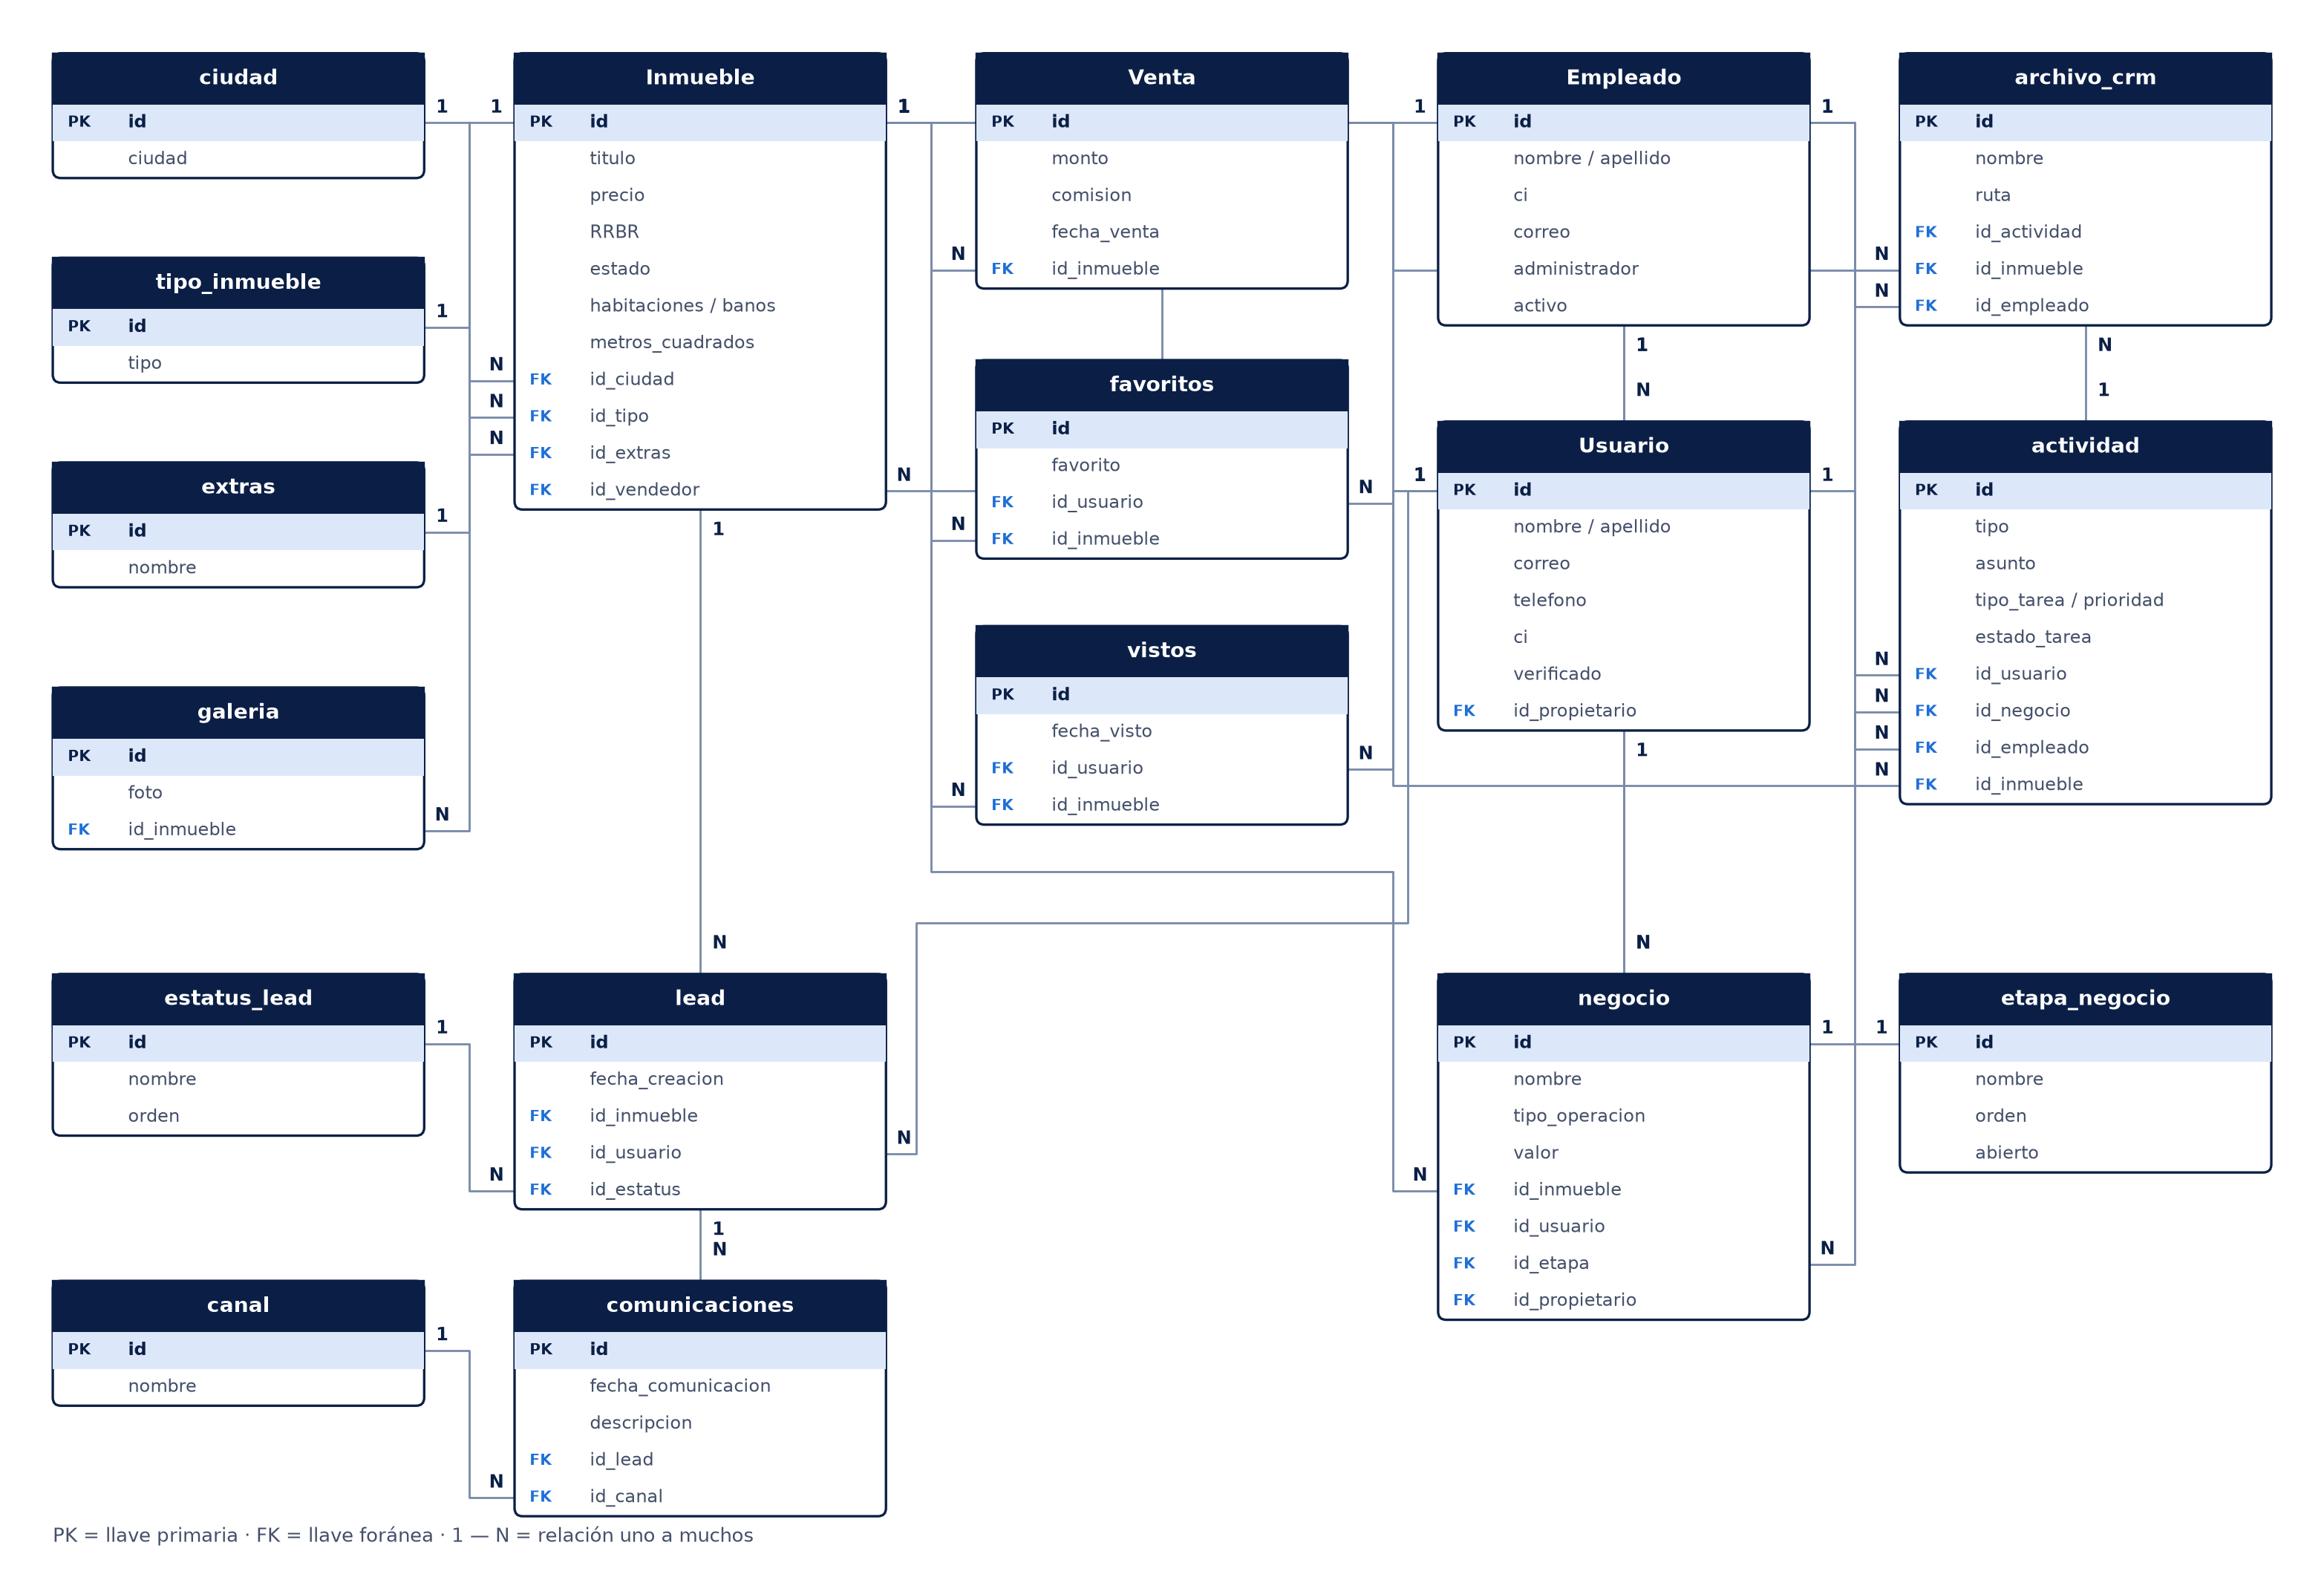
\includegraphics[width=\linewidth]{figuras/figura1.png}
\figurenote{Elaboración propia a partir del esquema implementado en PostgreSQL.}
\end{figure}

\subsubsection{Interfaces}

Las interfaces se diseñaron primero en Figma. Para el portal se priorizó la búsqueda y la presentación visual de los inmuebles. Para el CRM se definió un sistema de diseño de tono oscuro, con contenedores en azul pizarra (\#1a1c2e), botones activos en índigo (\#3b4cca), controles inactivos en gris azulado (\#2d325a), campos con bordes redondeados y formularios organizados en cuadrículas de dos columnas. Todos los módulos del CRM comparten la misma estructura: una barra lateral de navegación, pestañas para las vistas principales (\guillemotleft{}Todos\guillemotright{}, \guillemotleft{}Míos\guillemotright{}, \guillemotleft{}Sin asignar\guillemotright{}), un buscador con filtros y una tabla exportable.

\subsubsection{Seguridad}

Se diseñó un acceso por roles: administrador, vendedor y cliente. Al iniciar sesión, el servidor entrega un JSON Web Token (JWT), un pase firmado digitalmente que el navegador envía en cada petición para demostrar la identidad del usuario (Jones et al., 2015). Las contraseñas se almacenan cifradas con BCrypt, un algoritmo diseñado para resistir ataques de fuerza bruta (Provos \& Mazières, 1999). El cierre de sesión invalida los tokens anteriores y el servidor vuelve a validar el rol y el propietario de cada registro, de modo que un vendedor no puede modificar los negocios de otro aunque manipule la interfaz.

\subsection{Fase IV: Codificación}

Durante esta fase se programaron el portal, el CRM y la base de datos. El trabajo se organizó con Git en ramas por funcionalidad que luego se integraban a la rama principal, lo que permitió que los cuatro integrantes del equipo trabajaran en paralelo. La Tabla 7 resume las herramientas empleadas.

\begin{table}[htbp]
\caption{Tecnologías Empleadas en la Codificación}
\small
\begin{tabularx}{\linewidth}{>{\hsize=0.64\hsize}L>{\hsize=1.09\hsize}L>{\hsize=1.27\hsize}L}
\toprule
\textbf{Área} & \textbf{Tecnología} & \textbf{Uso en el proyecto} \\
\midrule
Interfaz & Vue 3, TypeScript, Vite y Vue Router & Portal y CRM; rutas públicas y rutas protegidas por rol. \\
Servidor & Spring Boot 4 (Java 17) y Maven & API REST con 21 controladores y reglas de negocio. \\
Persistencia & Spring Data JPA, Hibernate y PostgreSQL & Acceso a datos y filtros dinámicos con Criteria API. \\
Seguridad & Spring Security, JWT y BCrypt & Autenticación, roles y cifrado de contraseñas. \\
Reportes & Apache POI y OpenPDF & Exportación de tablas e informes a Excel y PDF. \\
Correo & Spring Mail (SMTP) & Códigos de verificación y correos a clientes con adjuntos. \\
Pruebas & JUnit con H2 y Vitest & Pruebas automatizadas del backend y del frontend. \\
\bottomrule
\end{tabularx}
\end{table}

\subsubsection{Base de Datos y Migraciones}

La base de datos se implementó en PostgreSQL alojado en Supabase (PostgreSQL Global Development Group, s.f.; Supabase, s.f.). Los cambios al esquema se aplicaron mediante ocho migraciones SQL numeradas: autenticación, bloqueo de la API pública de Supabase, recuperación de contraseña y sesiones, cédula del usuario, contactos, negocios e inmuebles con actividades, tareas y estadísticas, y características del inmueble. Al arrancar, el servidor verifica el esquema y advierte si falta alguna migración.

\subsubsection{Portal Web}

El portal se construyó como una aplicación de una sola página en Vue (Vue.js, s.f.). Incluye la página principal con el catálogo destacado, el buscador con filtros, la ficha de cada inmueble con galería, características, extras y mapa, y las pantallas de registro, verificación del correo, inicio de sesión, recuperación de contraseña y \guillemotleft{}Mi cuenta\guillemotright{}. La Figura 2 muestra la ficha de un inmueble.

\begin{figure}[htbp]
\caption{Ficha de un Inmueble en el Portal Web}
\centering
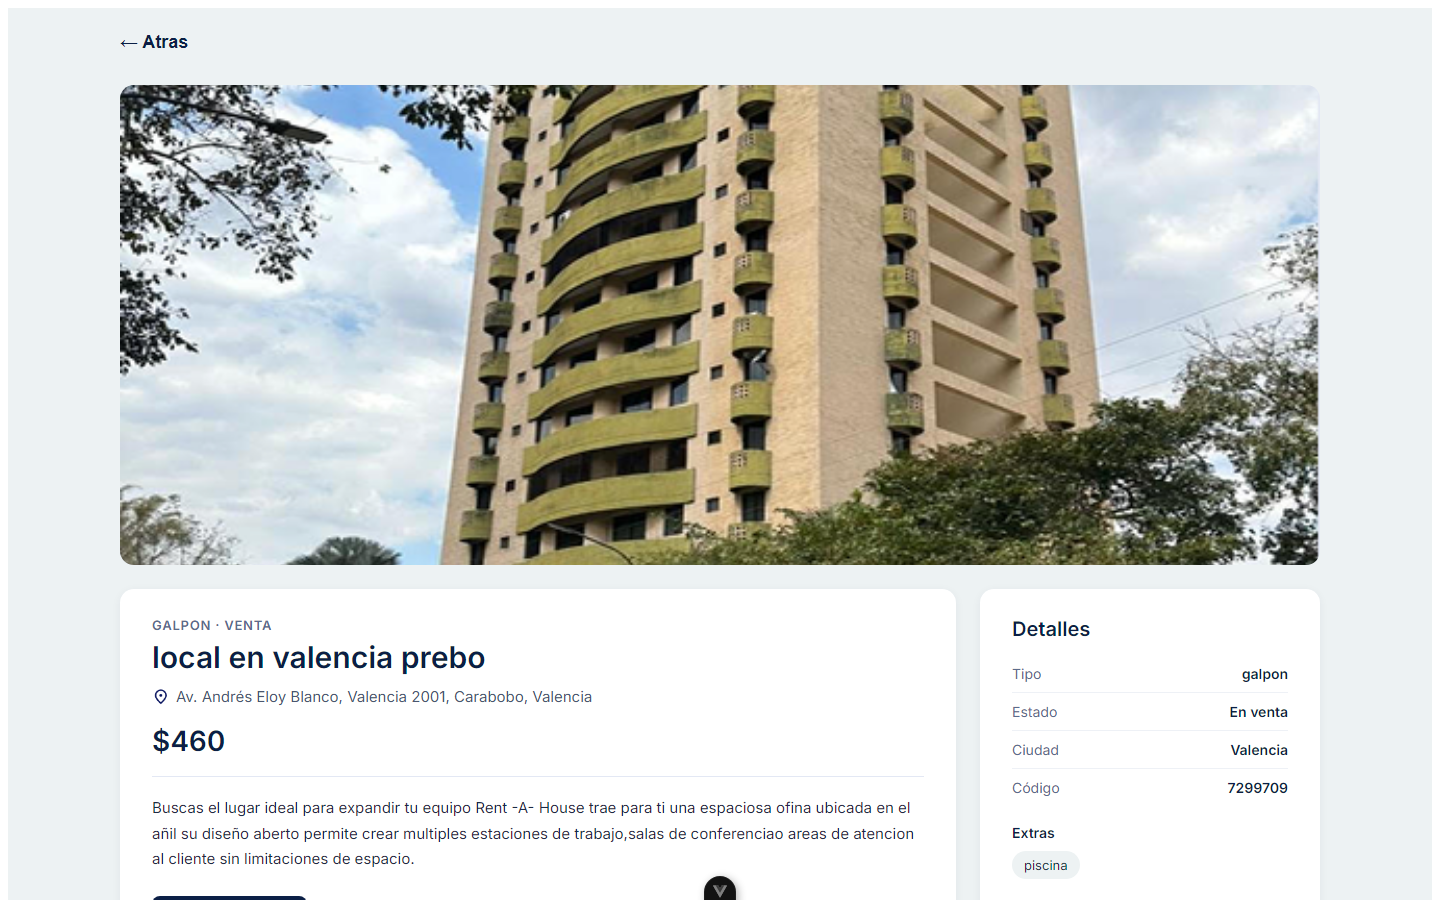
\includegraphics[width=\linewidth]{figuras/figura2.png}
\figurenote{Captura del entorno de prueba del sistema.}
\end{figure}

\subsubsection{Módulos del CRM}

El CRM se codificó en cinco módulos, accesibles desde una barra lateral tras iniciar sesión con una cuenta de empleado (Spring, s.f.):

\begin{enumerate}[label=\alph*)]
  \item \textbf{Contactos:} tabla con pestañas, buscador, filtros, edición de columnas y exportación. El registro de cada contacto se organiza en tres columnas: sus datos y accesos rápidos (nota, correo, llamada, tarea y reunión), su historial continuo y sus negocios, leads, adjuntos y actividad en el portal (Figura 3).
  \item \textbf{Negocios:} vista de tabla y vista de tablero, en la que cada etapa es una columna con el monto acumulado y las tarjetas se arrastran para cambiar de etapa (Figura 4).
  \item \textbf{Inmuebles:} inventario con estado comercial, dueño y asesor captador; la ficha incluye galería, características, mapa, documentos legales privados, negocios y clientes interesados.
  \item \textbf{Tareas:} tareas con tipo, estado, prioridad y vencimiento; las vencidas se calculan solas y, al completarse, el resultado queda como nota en el historial del cliente.
  \item \textbf{Estadísticas:} tarjetas de indicadores, gráficas del comportamiento del cliente y de las interacciones en el tiempo, tabla por inmueble y rendimiento por vendedor, con informe exportable (Figura 5).
\end{enumerate}

\begin{figure}[htbp]
\caption{Registro de un Contacto en el CRM}
\centering
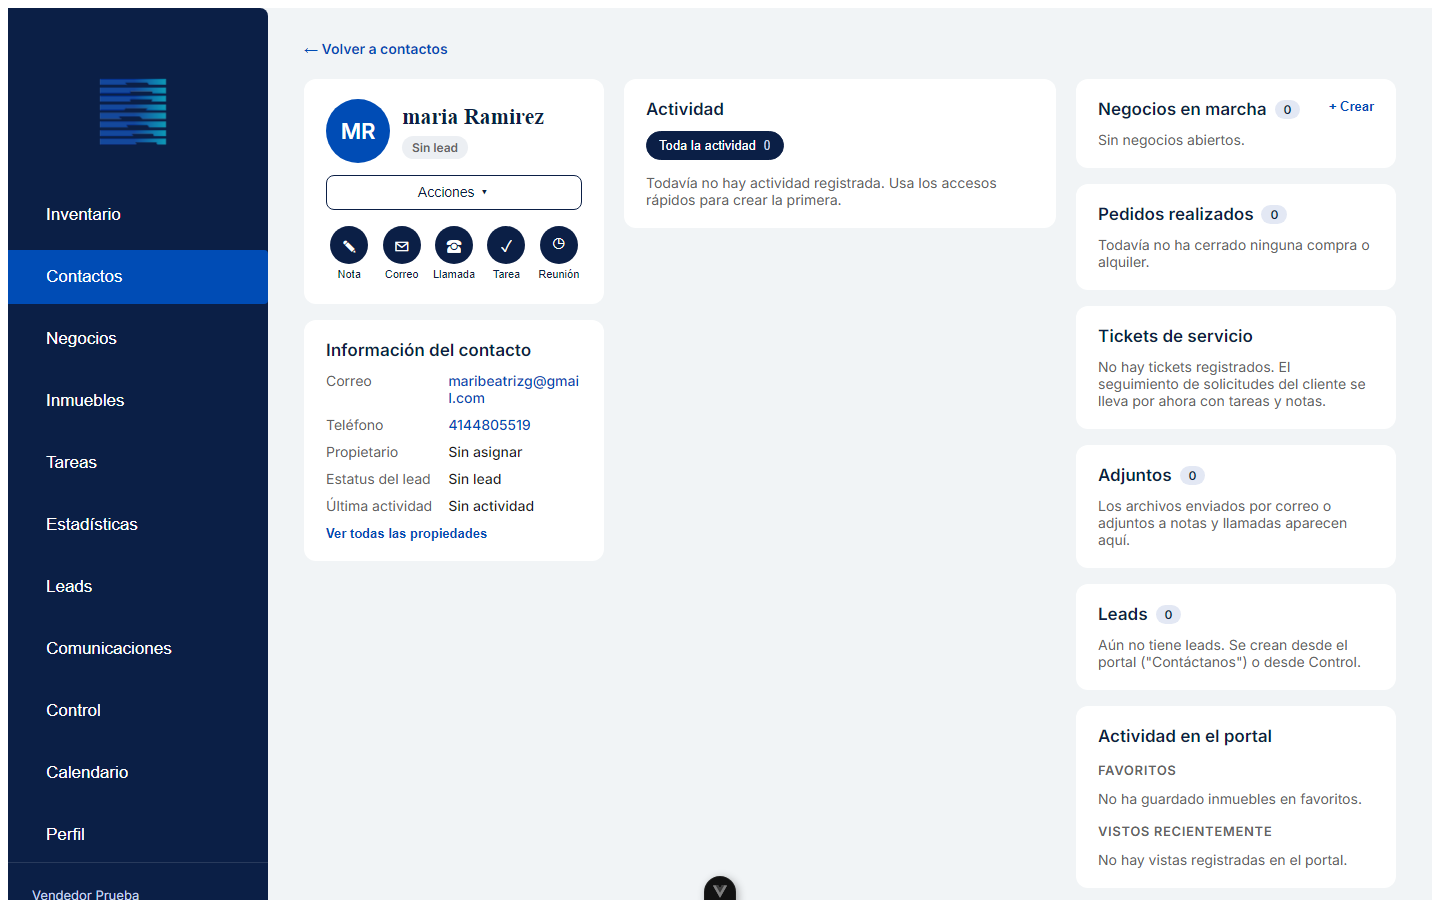
\includegraphics[width=\linewidth]{figuras/figura3.png}
\figurenote{Captura del entorno de prueba del sistema.}
\end{figure}

\begin{figure}[htbp]
\caption{Tablero de Negocios por Etapas del Embudo de Ventas}
\centering
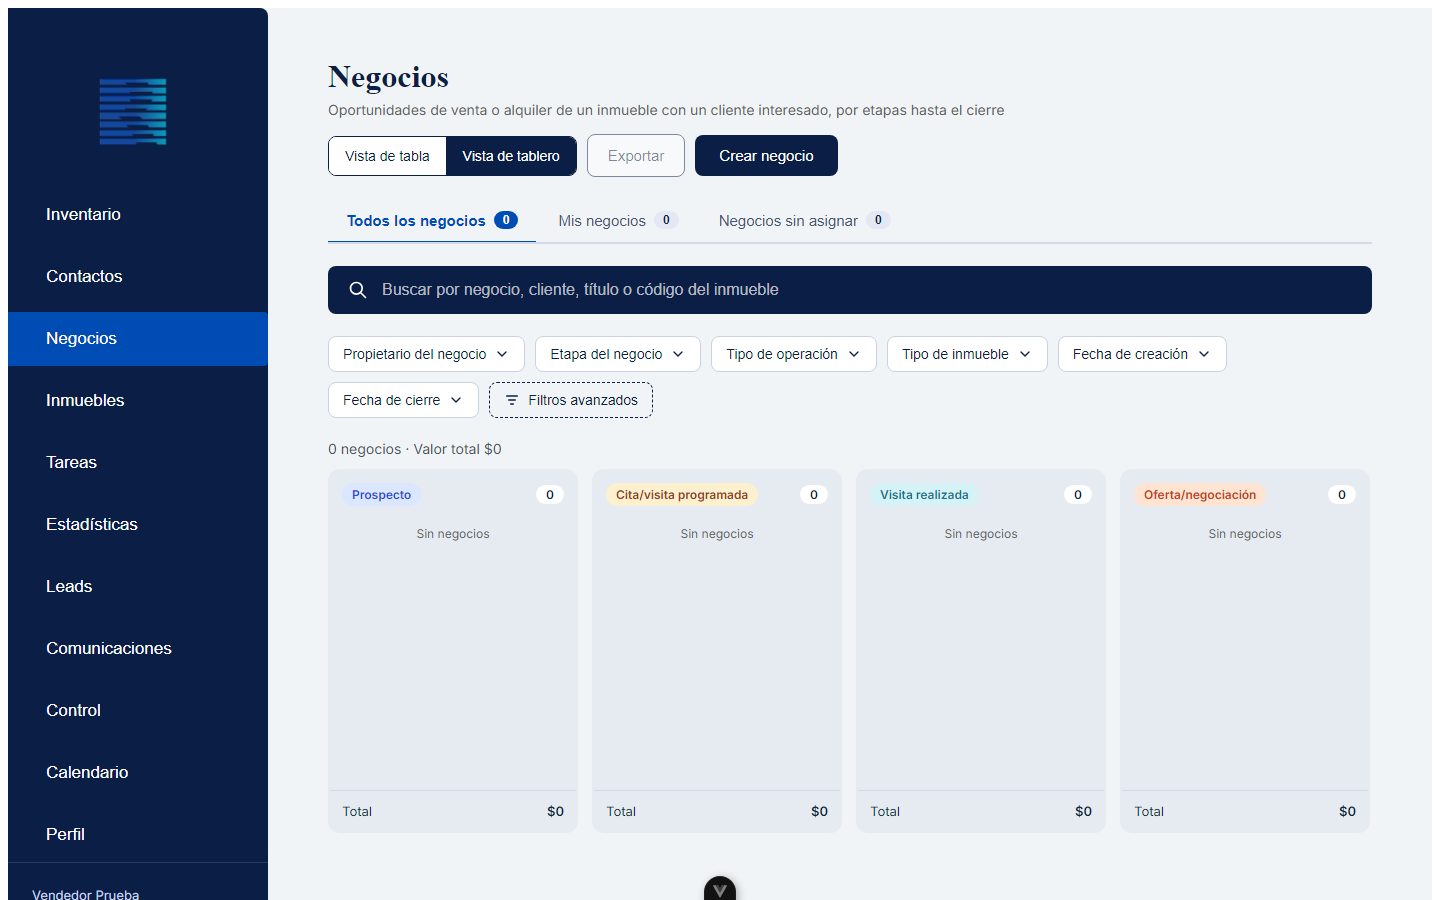
\includegraphics[width=\linewidth]{figuras/figura4.png}
\figurenote{Captura del entorno de prueba del sistema.}
\end{figure}

\begin{figure}[htbp]
\caption{Módulo de Estadísticas e Informes}
\centering
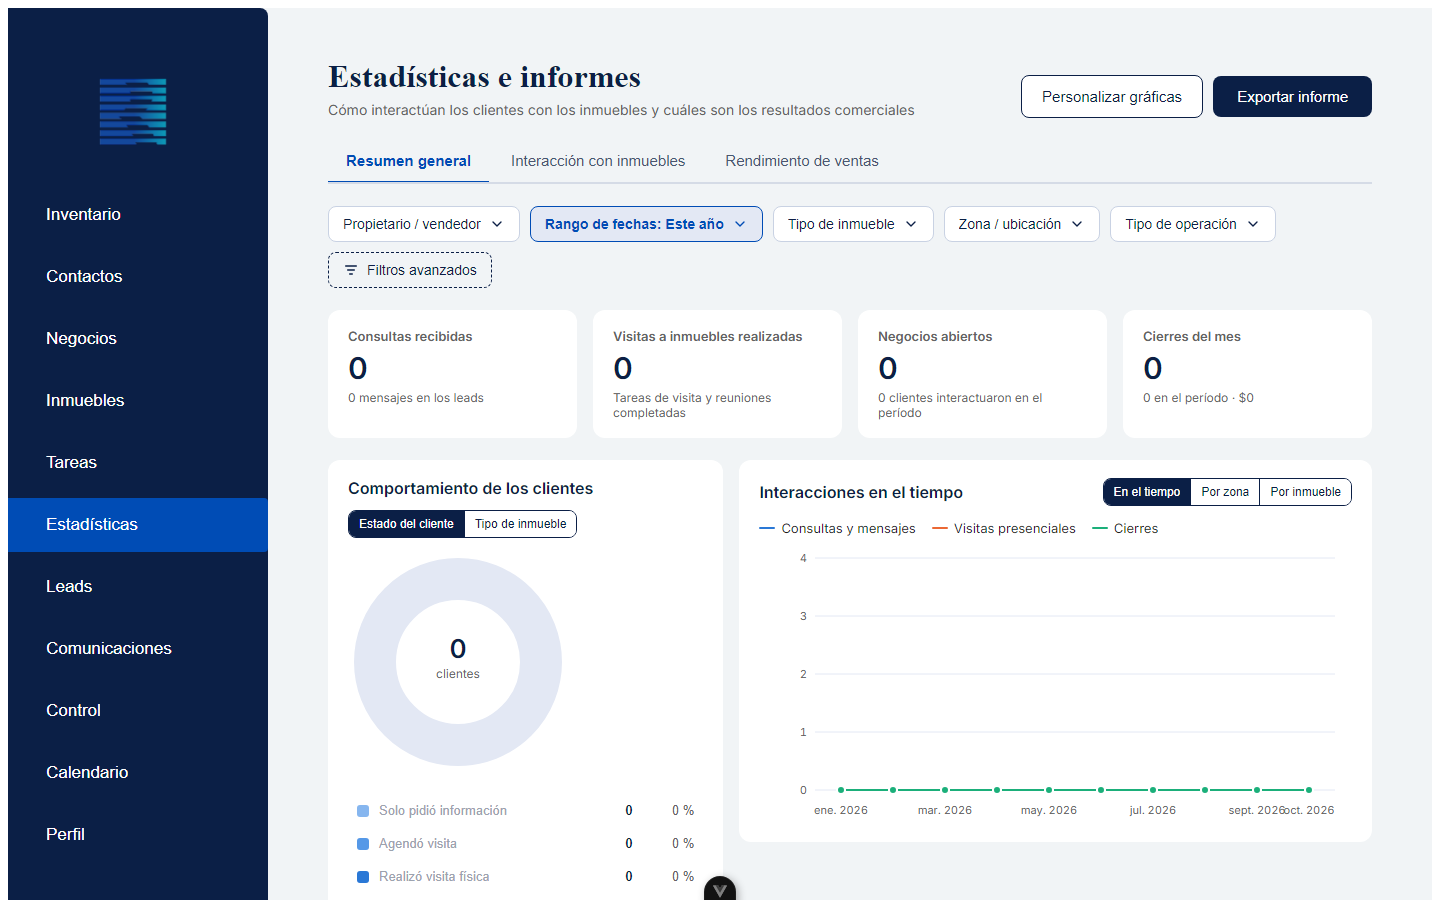
\includegraphics[width=\linewidth]{figuras/figura5.png}
\figurenote{Captura del entorno de prueba del sistema.}
\end{figure}

\subsubsection{Integración entre el Portal y el CRM}

La integración se logra porque ambas áreas comparten la misma base de datos. Cuando un cliente se registra en el portal, aparece de inmediato en la pestaña \guillemotleft{}Contactos sin asignar\guillemotright{} del CRM; cuando pide información sobre un inmueble, se crea un lead visible en su registro; y sus favoritos y vistas quedan como actividad en el portal. Un vendedor toma el contacto, crea un negocio con el inmueble de interés y lo acompaña por las etapas del embudo hasta el cierre. Cuando el inmueble se marca como vendido o alquilado, deja de mostrarse en el portal.

\subsection{Fase V: Evaluación}

La última fase comprobó que el sistema funciona como se especificó. Se aplicaron dos tipos de verificación: pruebas automatizadas, que ejecutan el código de forma repetible, y pruebas funcionales, en las que el equipo recorrió los casos de uso principales sobre el sistema en ejecución (Sommerville, 2016).

\subsubsection{Pruebas Automatizadas}

En el backend se escribieron 58 pruebas con JUnit que se ejecutan sobre una base de datos en memoria (H2) con las mismas consultas del sistema. Cubren la generación y validación de los tokens JWT, la protección de las rutas según el rol, el registro y la recuperación de cuentas, los filtros y exportaciones de contactos, el cambio de etapa de los negocios, el cálculo de tareas vencidas y las estadísticas. En el frontend se escribieron 36 pruebas con Vitest sobre los componentes y servicios principales. En la última ejecución, realizada el 23 de octubre de 2026, las 94 pruebas resultaron aprobadas, sin fallos ni errores.

\subsubsection{Pruebas Funcionales}

La Tabla 8 resume los casos de prueba funcionales ejecutados sobre el entorno de prueba con datos de demostración.

\begin{table}[htbp]
\caption{Casos de Prueba Funcionales}
\small
\begin{tabularx}{\linewidth}{>{\hsize=0.30\hsize}L>{\hsize=1.54\hsize}L>{\hsize=1.65\hsize}L>{\hsize=0.51\hsize}L}
\toprule
\textbf{N.º} & \textbf{Caso de prueba} & \textbf{Resultado esperado} & \textbf{Resultado} \\
\midrule
1 & Registro de un cliente en el portal con verificación por código. & Se crea el usuario y aparece en \guillemotleft{}Contactos sin asignar\guillemotright{}. & Aprobado \\
2 & Solicitud de información sobre un inmueble. & Se crea un lead visible en el registro del contacto. & Aprobado \\
3 & Asignación de un contacto a un vendedor. & El contacto pasa a \guillemotleft{}Mis contactos\guillemotright{} del vendedor. & Aprobado \\
4 & Cambio de etapa de un negocio en el tablero. & El negocio cambia de columna y el monto de cada etapa se actualiza. & Aprobado \\
5 & Vendedor intenta modificar un negocio ajeno. & El servidor rechaza la operación. & Aprobado \\
6 & Tarea con fecha de vencimiento pasada. & Se marca automáticamente como vencida. & Aprobado \\
7 & Inmueble marcado como vendido. & Deja de aparecer en el portal. & Aprobado \\
8 & Exportación de tablas e informe de estadísticas. & Se descargan archivos Excel y PDF con los datos filtrados. & Aprobado \\
9 & Cierre de sesión y reutilización del token anterior. & El token anterior deja de ser válido. & Aprobado \\
\bottomrule
\end{tabularx}
\end{table}

\subsubsection{Cumplimiento de los Requerimientos}

Al contrastar el sistema con los requerimientos de la Fase II, los diez requerimientos funcionales quedaron implementados y verificados. En cuanto a los no funcionales, la seguridad se cubrió con roles, JWT, BCrypt y validación en el servidor; la integridad, con las restricciones de la base de datos; la mantenibilidad, con la organización por capas y las migraciones versionadas; y la verificabilidad, con las pruebas automatizadas de ambas capas.

\subsubsection{Limitaciones}

Las pruebas se realizaron en un entorno de prueba con datos de demostración, por lo que aún debe medirse el comportamiento del sistema con el volumen real de la inmobiliaria y con varios asesores trabajando al mismo tiempo. Asimismo, algunas funciones, como un módulo de tickets de servicio y un calendario propio, se cubren por ahora con tareas y notas.

\section{Conclusiones}

El proyecto cumplió su objetivo general: Rifat Richani Bienes Raíces cuenta con un sistema que conecta su portal web con un CRM y centraliza la gestión de contactos, negocios, inmuebles, tareas y estadísticas sobre una sola base de datos.

El \textbf{diagnóstico} permitió identificar que el problema no estaba en atraer clientes, pues el portal ya lo hacía, sino en lo que ocurría después del primer contacto: información dispersa, falta de responsables y ausencia de métricas. La \textbf{determinación} de requerimientos tradujo esas necesidades en diez requerimientos funcionales y en un embudo de siete etapas que refleja el proceso real de una venta inmobiliaria.

El \textbf{diseño} en tres capas, con una base de datos relacional normalizada de 18 tablas y un esquema de seguridad por roles, dio al sistema una estructura ordenada y extensible, lo que permitió agregar los módulos de negocios, tareas y estadísticas sin alterar las tablas originales. La \textbf{codificación} con Vue 3, Spring Boot y PostgreSQL produjo un portal y un CRM funcionales e integrados, en los que el cliente que se registra en el portal aparece al instante en el CRM.

Por último, la \textbf{evaluación} mediante pruebas automatizadas y funcionales confirmó que el sistema cumple los requerimientos establecidos. Con ello, cada cliente de la inmobiliaria tiene ahora un responsable, un historial y un seguimiento medible, y la gerencia dispone de datos para tomar decisiones.

\section{Recomendaciones}

Se recomienda poner el sistema en producción de forma gradual, comenzando con un grupo reducido de asesores, y capacitar al personal en el uso del CRM. También se sugiere realizar pruebas de carga con el volumen real de datos, programar respaldos periódicos de la base de datos y evaluar a futuro la incorporación de un módulo de tickets, un calendario integrado y la conexión con WhatsApp para registrar las conversaciones en el historial del cliente.

\newpage
\section{Referencias}

\begingroup
\setlength{\parindent}{-0.5in}
\setlength{\leftskip}{0.5in}

Buttle, F., \& Maklan, S. (2019). \textit{Customer relationship management: Concepts and technologies} (4.ª ed.). Routledge. \url{https://doi.org/10.4324/9781351016551}

Codd, E. F. (1970). A relational model of data for large shared data banks. \textit{Communications of the ACM, 13}(6), 377–387. \url{https://doi.org/10.1145/362384.362685}

Elmasri, R., \& Navathe, S. B. (2016). \textit{Fundamentals of database systems} (7.ª ed.). Pearson.

Fielding, R. T. (2000). \textit{Architectural styles and the design of network-based software architectures} [Tesis doctoral, University of California, Irvine]. \url{https://ics.uci.edu/~fielding/pubs/dissertation/top.htm}

Halligan, B., \& Shah, D. (2014). \textit{Inbound marketing: Attract, engage, and delight customers online} (Ed. rev.). Wiley.

Hernández Sampieri, R., Fernández Collado, C., \& Baptista Lucio, P. (2014). \textit{Metodología de la investigación} (6.ª ed.). McGraw-Hill.

Jones, M., Bradley, J., \& Sakimura, N. (2015). \textit{JSON Web Token (JWT)} (RFC 7519). Internet Engineering Task Force. \url{https://doi.org/10.17487/RFC7519}

Kotler, P., \& Keller, K. L. (2016). \textit{Dirección de marketing} (15.ª ed.). Pearson.

PostgreSQL Global Development Group. (s.f.). \textit{PostgreSQL documentation}. \url{https://www.postgresql.org/docs/}

Pressman, R. S., \& Maxim, B. R. (2020). \textit{Software engineering: A practitioner’s approach} (9.ª ed.). McGraw-Hill Education.

Provos, N., \& Mazières, D. (1999). A future-adaptable password scheme. En \textit{Proceedings of the 1999 USENIX Annual Technical Conference} (pp. 81–91). USENIX Association.

Silberschatz, A., Korth, H. F., \& Sudarshan, S. (2020). \textit{Database system concepts} (7.ª ed.). McGraw-Hill Education.

Sommerville, I. (2016). \textit{Software engineering} (10.ª ed.). Pearson.

Spring. (s.f.). \textit{Spring Boot reference documentation}. \url{https://docs.spring.io/spring-boot/}

Supabase. (s.f.). \textit{Supabase documentation}. \url{https://supabase.com/docs}

Vue.js. (s.f.). \textit{Vue.js guide}. \url{https://vuejs.org/guide/}

\endgroup

\end{document}
